% 초안 v4 — 쉬운 말 판. XeLaTeX + kotex (Tectonic: tectonic -o docs/paper docs/paper/draft_v4.tex). 내용은 DRAFT_v4.md 와 같다.
\documentclass[10pt,a4paper]{article}
\usepackage{kotex}
\IfFontExistsTF{Noto Sans CJK KR}{\setmainhangulfont{Noto Sans CJK KR}}{\setmainhangulfont{Malgun Gothic}}
\usepackage[margin=20mm]{geometry}
\usepackage{amsmath,amssymb}
\usepackage{booktabs,array}
\usepackage{graphicx}
\usepackage[colorlinks=true,linkcolor=blue,citecolor=blue,urlcolor=blue]{hyperref}
\usepackage{xcolor}
\newcommand{\todo}[1]{\textcolor{red}{[#1]}}
\graphicspath{{./}}

\title{삭제 요청으로 깨어나는 백도어를 학습 중에 찾아 걷어내기:\\서로 지우는 기여의 탐지}
\author{(저자)}
\date{초안 v4 (쉬운 말 판), 2026-10-13}

\begin{document}
\maketitle

\section*{용어}
\begin{tabular}{p{0.3\linewidth}p{0.66\linewidth}}\toprule
말 & 뜻\\\midrule
심는 클라이언트 & 트리거가 붙은 입력을 타깃 클래스로 분류하도록 모델을 미는 공격자. 논문 설정에서 넷(0--3)\\
숨기는 클라이언트 & 심는 쪽의 효과를 같은 양만큼 되밀어 모델을 깨끗하게 보이게 하는 공격자. 한 명(4). 나중에 삭제를 요청한다\\
소유자 & 한 클래스(3)의 데이터 90\%를 가진 \emph{정상} 클라이언트(19). non-IID 조건에만 있다\\
공개 입력 & 서버가 가진 라벨 없는 시험 이미지 500장\\
누적 영향 $P_j(c)$ & 클라이언트 $j$가 참여한 라운드마다, $j$의 갱신 하나가 공개 입력 위에서 클래스 $c$의 로그확률 평균을 얼마나 바꿨는지를 더한 값. 양수면 올렸고 음수면 내렸다\\
상쇄율 $H(c)$ & 클래스 $c$에서 모든 클라이언트의 누적 영향을 더한 합의 크기를, 각자의 영향 크기의 합으로 나눠 1에서 뺀 것. 모두 같은 방향이면 0, 서로 지워서 합이 0이면 1\\
가장 내린 클라이언트 & 클래스 $c$의 누적 영향이 가장 음수인 클라이언트\\
유의하게 올린 클라이언트들 & 누적 영향이 나머지의 중앙값보다 MAD의 2배 넘게 큰 클라이언트들\\
공모 & 한 클래스에서 유의하게 올린 클라이언트가 둘 이상이고, 한 명이 올린 몫의 6할을 넘지 않으며, 가장 내린 클라이언트가 그 합을 거의 다 지우는 상태\\
경보 & 같은 클래스가 세 라운드 연속 공모로 판정되는 것\\
\bottomrule\end{tabular}

\begin{abstract}
연합학습 서버가 삭제 요청을 받으면 저장해 둔 그 클라이언트의 갱신을 모델에서 걷어낸다. 최근 공격(FUBA, BadFU)은 이것을 이용한다. 공격자 몇 명이 백도어를 심고, 다른 한 명이 같은 양만큼 되밀어 학습이 끝난 모델을 깨끗하게 만든 뒤, 되밀던 사람이 삭제를 요청하면 백도어가 드러난다. 이 논문은 이런 공격이 학습 중에 반드시 남기는 흔적을 찾는다. 심는 쪽과 숨기는 쪽은 같은 입력에 서로 반대되는 학습 신호를 보내므로, 라운드마다 각 클라이언트의 갱신이 공개 입력 위에서 타깃 클래스의 확률을 얼마나 바꾸는지를 더해 보면, 한 클래스에서만 ``여럿이 크게 올리고 한 명이 그만큼 내려서 합은 0''인 모양이 나온다. 정상 학습에서는 이 모양이 나오지 않는다. 데이터가 많은 정상 클라이언트는 자기 클래스를 크게 올리지만 그것을 되미는 사람이 없고, 정상 클라이언트는 남이 올린 것을 되밀 이유가 없기 때문이다. 서버는 라운드마다 참여자 수만큼의 순전파로 이 양을 누적하고, 위 모양이 세 라운드 연속 보이면 경보를 내며, 경보에는 타깃 클래스·숨기는 클라이언트·심는 클라이언트들·되돌아갈 라운드가 함께 나온다. 대응은 그 라운드의 모델로 돌아가 공모자를 뺀 채 이어 학습하는 것이다. FUBA 논문 설정(클라이언트 20, 공격자 5, 100 라운드, 참여율 0.4, IID·non-IID 각 3 시드)에서 6 궤적 모두 11--16 라운드에 경보가 났고, 숨기는 클라이언트와 심는 클라이언트 넷을 정확히 가리켰으며, 소유자를 한 번도 공격자로 보지 않았다. 공모자를 뺀 재학습은 공격 성공률 0.5--0.6\%, 정확도 99\%다. 갱신 하나의 크기나 방향을 보는 기존 방어는 소유자를 같이 잡거나 심는 클라이언트를 가장 정상으로 보았다.
\end{abstract}

\section{문제: 삭제가 백도어를 켠다}
연합학습에서 서버는 클라이언트들의 갱신을 평균해 모델을 만든다. 삭제권을 지키려면 특정 클라이언트의 몫을 모델에서 걷어내야 하므로, 연합 언러닝 서버는 라운드별 갱신을 저장해 둔다.

공격은 이 걷어내기를 거꾸로 쓴다. FUBA를 예로 들면 다음과 같다.
\begin{enumerate}
\item 심는 클라이언트 넷은 트리거 생성기를 함께 학습하며, 트리거가 붙은 입력이 클래스 8로 분류되도록 갱신을 보낸다.
\item 숨기는 클라이언트 한 명은 전역 모델이 깨끗한 모델처럼 보이도록 되미는 갱신을 보낸다(저자 표현으로 model-consistency 손실; 본문은 초록·슬라이드로 확인).
\item 서버가 평균을 내면 둘이 지워져 학습이 끝난 모델은 깨끗하다. 트리거 입력의 공격 성공률이 3--8\%다(표~\ref{tab:attack}).
\item 숨기는 클라이언트가 삭제를 요청한다. 서버가 그 갱신을 걷어내면 되밀던 힘이 사라지고 공격 성공률이 46--93\%가 된다.
\end{enumerate}
서버가 요청을 더 정확히 이행할수록 공격은 더 잘 된다. 심는 클라이언트들을 남긴 채 처음부터 다시 학습해도 백도어 모델이 나온다($K=8$ 예비, 30--44\%). 즉 ``요청자를 잘 지우는 것''은 답이 아니다. 심는 쪽을 찾아 걷어내야 한다.

\section{기존 방어가 못 보는 이유}
기존 연합학습 방어는 갱신 \emph{하나}의 성질을 본다. 크기(노름, Krum 거리), 방향(서버 기준과의 코사인), 출력층의 에너지 분포. 또는 갱신들끼리 얼마나 닮았는지를 본다(FoolsGold). 언러닝 전용 방어(MASA, SubID)는 삭제를 요청한 \emph{한 명}의 갱신만 본다.

이 공격에서는 두 가지가 동시에 일어난다(표~\ref{tab:baselines}).
\begin{itemize}
\item 숨기는 클라이언트의 갱신은 크다. 크기 기준은 그를 잡는다. 그러나 데이터가 많은 정상 클라이언트(소유자)의 갱신도 커서 함께 잡힌다(소유자의 $z$ 3.8--65).
\item 심는 클라이언트들의 갱신은 방향이 평범하다. 20명 중 가장 중심에 있다(평균 순위 18.5/20). 방향 기준으로는 보이지 않는다.
\end{itemize}
문제의 본질은 갱신 하나가 아니라 \emph{둘 사이의 관계}다. 심는 쪽이 올린 만큼 숨기는 쪽이 내린다. 한 명씩 보면 아무 이상이 없고, 둘을 같은 저울에 올려야 보인다.

\section{공격이 남기는 흔적}
\subsection{왜 흔적이 남는가}
모델의 출력은 클래스별 로그확률이다. 라운드 $t$에서 클라이언트 $j$의 갱신을 전역 모델에 더하면 출력이 조금 바뀐다. 이 변화를 공개 입력 500장에서 평균하면 ``$j$의 이번 갱신이 클래스 $c$를 얼마나 올렸나''가 된다. 순전파 한 번이면 된다. 이것을 $j$가 참여한 라운드마다 더한 것이 \emph{누적 영향} $P_j(c)$다.
\begin{equation}
P_j(c)=\sum_{t:\,j\in P_t}\ \operatorname{mean}_{x\in X_p}\big[f_c(x;\theta_{t-1}+U_j^t)-f_c(x;\theta_{t-1})\big]
\end{equation}
($f_c$: 클래스 $c$의 로그확률, $U_j^t$: 집계 가중치를 곱한 갱신, $X_p$: 공개 입력.)

심는 클라이언트는 트리거 입력에서 클래스 8을 올려야 하므로 공개 입력에서도 클래스 8을 조금 올린다. 숨기는 클라이언트는 전역 모델 전체를 깨끗한 쪽으로 되밀므로 공개 입력에서 클래스 8을 크게 내린다. 둘의 합이 0에 가까워야 모델이 깨끗해 보이고, 둘의 크기가 커야 삭제 뒤에 백도어가 켜진다. 그러므로 공격이 성공하려면 클래스 8에서 다음 네 가지가 동시에 성립해야 한다.
\begin{enumerate}
\item 모든 클라이언트의 누적 영향을 더하면 0에 가깝다.
\item 그런데 각자의 영향은 크다.
\item 가장 내린 클라이언트는 한 명이다(숨기는 클라이언트).
\item 유의하게 올린 클라이언트는 여럿이다(심는 클라이언트들).
\end{enumerate}

\subsection{실제로 그렇게 보이는가 (R-012, 그림~\ref{fig:push})}
논문 설정 6 궤적의 학습 끝에서 클래스 8의 누적 영향: 숨기는 클라이언트 4는 $-29.7\ldots-39.4$(6 궤적 모두 최솟값), 심는 클라이언트 0--3은 각자 $+3.3\ldots+16.3$, 정상은 $-3.9\ldots+4.9$, 소유자 19는 $+0.2\ldots+3.8$. 합의 크기는 각자 크기 합의 7--16\%다. 네 조건이 전부 성립한다.
\begin{figure}[t]\centering
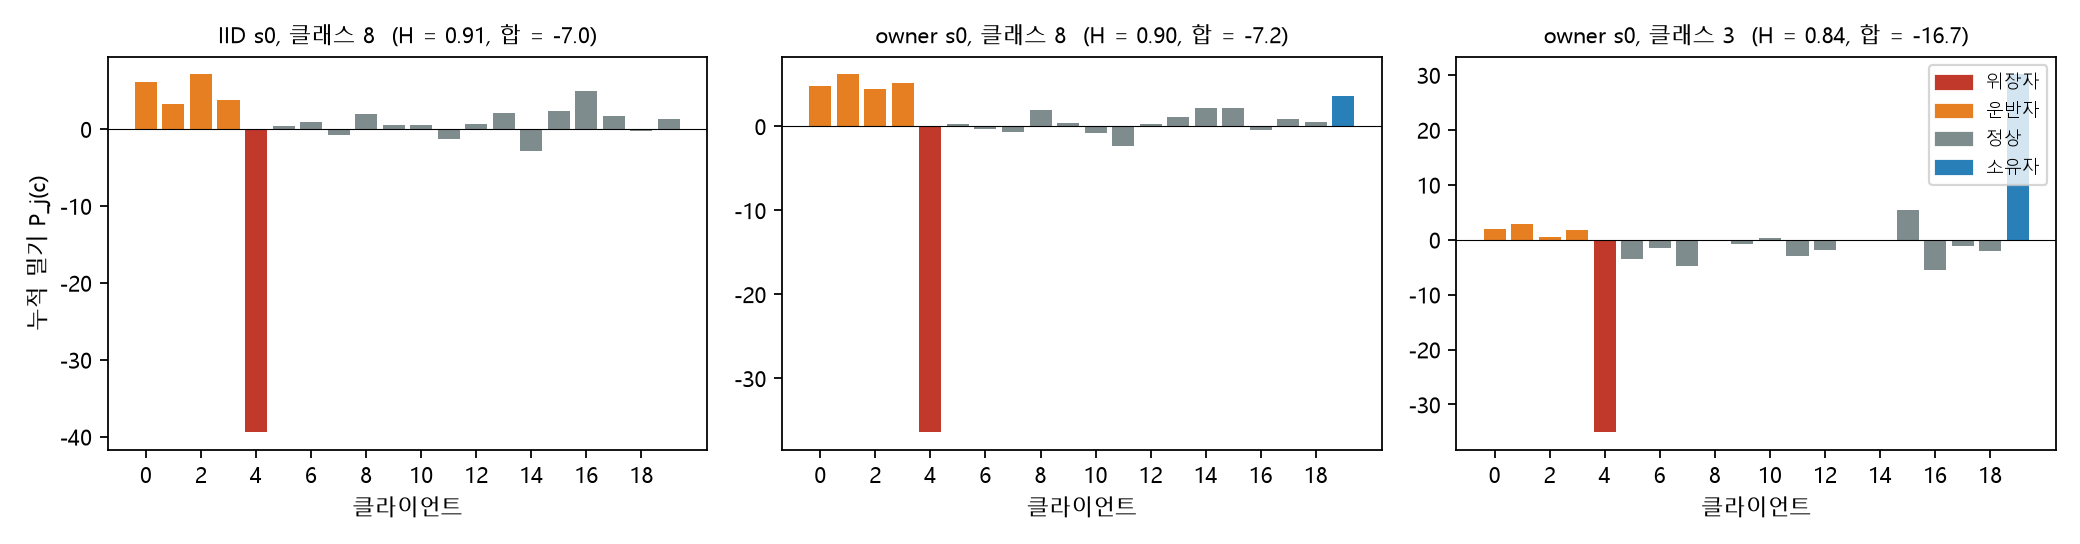
\includegraphics[width=\linewidth]{fig_push_bar.png}
\caption{학습 끝의 누적 영향. 왼쪽·가운데: 클래스 8---심는 넷(주황)이 올리고 숨기는 한 명(빨강)이 내린다. 오른쪽: non-IID 조건의 클래스 3---소유자(파랑) 한 명이 올리고 숨기는 클라이언트가 내린다. 내리는 사람은 같지만 올리는 사람 수가 다르다.}
\label{fig:push}
\end{figure}

\subsection{왜 정상 학습에는 없는가}
정상 클라이언트의 갱신은 자기 데이터의 손실만 줄인다. 자기가 가진 클래스를 올리고, 남이 올린 것을 되밀 이유가 없다. IID면 모두 비슷하게 올리므로 합이 크고 상쇄율은 0에 가깝다. non-IID면 소유자 한 명이 자기 클래스를 크게 올리고 나머지는 거의 안 움직이므로 역시 합이 크다. ``한 명이 크게 내리고 그 크기가 여럿이 올린 합과 같다''는 모양은 데이터 분포의 차이로는 생기지 않는다. 그것은 다른 사람들의 학습을 \emph{되돌리는} 행동이고, 정직한 손실 함수에는 그런 항이 없다.

\subsection{소유자와 어떻게 구분하는가}
non-IID 조건에서 숨기는 클라이언트는 클래스 8만이 아니라 소유자가 가르친 클래스 3도 내린다(소유자 $+30$, 숨기는 클라이언트 $-35$). 전역 모델의 변화 전체를 되돌리기 때문이다. 그래서 클래스 3도 ``합은 0, 가장 내린 사람 한 명''이다. 차이는 올린 쪽이다. 클래스 8은 심는 넷이 나눠 올리고(한 명의 최대 몫 0.31--0.54), 클래스 3은 소유자 한 명이 거의 전부 올린다(몫 $>0.6$). 여럿이 나눠 올리면 공모, 한 명이 올리면 정상 큰손으로 본다. 소유자는 손대지 않는다.

\section{방법}
\subsection{서버가 하는 일 (라운드마다)}
\begin{enumerate}
\item 참여자 $j$마다: 전역 모델에 $j$의 갱신(집계 가중치 적용)을 더한 모델로 공개 입력 500장을 순전파하고, 클래스별 로그확률 평균의 변화를 $P_j(\cdot)$에 더한다. 순전파는 참여자 수 $+1$번.
\item 클래스 $c$마다 네 수를 계산한다. 상쇄율 $H(c)=1-|\sum_jP_j(c)|/\sum_j|P_j(c)|$; 가장 내린 클라이언트와 그 $z$ 점수 $z_j(c)=(P_j(c)-\operatorname{median}_iP_i(c))/\operatorname{MAD}_iP_i(c)$; 유의하게 올린 클라이언트들 $\{j: z_j(c)>2\}$; 올린 몫 중 최대 한 명의 비율.
\item 클래스 $c$를 \textbf{공모}로 판정한다 $\Leftrightarrow$ $H(c)\ge0.8$, 가장 내린 클라이언트의 $z\le-3$, 유의하게 올린 클라이언트가 2명 이상, 그중 한 명의 몫이 0.6 이하. 올린 사람이 한 명이거나 몫이 0.6을 넘으면 \textbf{정상 큰손}(소유자형)으로 보고 손대지 않는다. 올린 사람이 없으면 \textbf{내리기만 있음}으로 적어 두기만 한다(숨기는 클라이언트는 타깃이 아닌 클래스도 내리므로 이런 클래스가 몇 개 생긴다).
\item 같은 클래스가 3 라운드 연속 공모이면 \textbf{경보}. 판정은 5 라운드부터, 두 번 이상 참여한 클라이언트만 후보로 둔다.
\end{enumerate}
\subsection{경보가 주는 것}
타깃 클래스 $c^*$, 숨기는 클라이언트 후보(가장 내린 사람), 심는 클라이언트 후보(연속 판정 동안 한 번이라도 유의하게 올린 사람들), 되돌아갈 라운드(경보 전에 $H(c^*)$가 0.8 아래였던 마지막 라운드).
\subsection{대응}
되돌아갈 라운드의 전역 모델에서 시작해, 숨기는 클라이언트와 심는 클라이언트들을 뺀 채 남은 라운드를 이어 학습한다. 저자의 학습 코드를 그대로 쓰고 시작 모델과 제외 목록만 바꾼다. 요청이 학습이 끝난 뒤에 오면 저장된 갱신 위에 같은 계산을 사후에 하면 같은 판정이 나오고, 공모자를 뺀 재학습으로 요청을 이행한다.
\subsection{문턱값과 비용}
상쇄율 0.8, 내린 $z$ $-3$, 올린 $z$ 2, 올린 사람 2명 이상, 최대 몫 0.6, 연속 3 라운드, 시작 5 라운드(민감도 \S\ref{sec:sens}). 비용은 라운드당 (참여자 수 $+1$)$\times$500장 순전파. 모델을 새로 만들지 않고 라벨·트리거·역할 정보가 필요 없다. 대응은 남은 라운드(87--93) 학습이다.

\section{왜 피할 수 없는가}
\paragraph{공격의 필요조건이 곧 판정의 양성 조건이다.} 학습 끝 모델이 트리거 입력에서 깨끗하려면 트리거 입력 위에서 심는 쪽의 영향과 숨기는 쪽의 영향이 지워져야 한다. 삭제 뒤에 켜지려면 숨기는 쪽의 영향이 커야 한다. 이 상쇄가 공개 입력에도 일정 비율로 새면(FUBA는 전역 모델 전체를 되밀므로 샌다; 실측 R-012), 공개 입력 위의 누적 영향에서 \S3.1의 네 조건이 성립한다. 이것이 공모 판정이다. 1차 근사로 $P_j(c)$의 라운드 항은 $\langle U_j^t,\nabla_\theta f_c\rangle$의 평균이고 전역 갱신의 변화는 참여자 항의 합이므로, ``모델이 깨끗하다''는 ``항들의 합이 0''이고 ``삭제로 켜진다''는 ``한 항이 크다''다.
\paragraph{정상에서 거짓 경보가 나려면} 어떤 클라이언트가 나머지보다 MAD 3배 넘게 내리면서, 동시에 둘 이상이 MAD 2배 넘게 올리고, 그 합이 서로 지워야 한다. 정상 영향이 독립이면 이 셋의 동시 확률은 각각의 꼬리 확률의 곱보다 작다. 소유자는 자기 클래스를 올리므로 ``가장 내린 사람''이 될 수 없다. \todo{공격 없는 궤적의 실측 R-015 예정}
\paragraph{공격자가 피하려면.} (a) 되밀기를 여러 명에 나누면 가장 내린 사람이 집합이 된다---$z\le-3$인 사람 전부를 내린 쪽으로 보면 같은 규칙이 적용된다 \todo{R-016 예정}. (b) 되밀기를 약하게 하면 학습 중 공격 성공률이 올라 숨지 못한다. (c) 상쇄를 트리거 입력에만 가두고 공개 입력에 새지 않게 하면 이 방법은 보지 못한다---이것이 경계이며, 그때는 요청 시점에 지울 입력을 포함한 집합에서 조금 빼 보는 심사(R-009의 flow $z$, 숨기는 클라이언트 3/3, 소유자 $z$ 0)가 보완한다. BadFU의 노트북 15 라운드 궤적이 이 경우다(R-017: 경보 없음). (d) 심는 사람을 아주 많이 두어 각자의 몫을 작게 하면 올린 사람 집합이 비지만, 합은 여전히 숨기는 쪽을 지워야 하므로 상쇄율과 내린 $z$는 남는다(내리기만 있음으로 보고됨).

\section{평가}
\paragraph{설정.} FUBA 저자 코드 그대로. MNIST, LeNet, 클라이언트 20, 심는 클라이언트 0--3, 숨기는 클라이언트 4, 100 라운드(웜업 5), 참여율 0.4. 조건: IID, non-IID(클라 19가 클래스 3의 90\%). 시드 3. 공개 입력: 시험 집합 500장. 서버는 역할·타깃·트리거를 모른다. 역할은 채점에만 쓴다.

\begin{table}[t]\centering\small
\caption{공격은 재현된다(R-006). 정확도/공격 성공률(\%). 숨기는 클라이언트를 전량 빼면 모델이 무너진다(정확도 9.7\%, R-007).}
\label{tab:attack}
\resizebox{\linewidth}{!}{%
\begin{tabular}{lllll}\toprule
 & 학습 끝 & 숨기는 클라이언트 20\% 제거 & 정상 1명 제거 & 심는 클라이언트 1명 제거\\\midrule
IID s0·s1·s2 & 98.8/7.4 · 98.7/3.1 · 98.6/4.8 & 68.7/92.6 · 97.6/46.2 · 86.6/82.3 & 97.8/3.9 · 96.5/2.4 · 94.8/4.9 & 98.3/0.6 · 98.1/0.6 · 97.3/0.6\\
non-IID s0·s1·s2 & 98.2/7.8 · 98.3/3.6 · 98.1/5.7 & 73.1/85.7 · 96.7/50.0 · 82.5/78.9 & 96.1/9.8 · 95.8/5.8 · 96.0/4.4 & 98.0/1.4 · 96.5/0.2 · 94.5/0.2\\
성공률 평균 (IID / non-IID) & 5.1$\pm$1.8 / 5.7$\pm$1.7 & 73.7$\pm$19.9 / 71.5$\pm$15.5 & 3.7$\pm$1.0 / 6.7$\pm$2.3 & 0.6$\pm$0.0 / 0.6$\pm$0.6\\
\bottomrule\end{tabular}}
\end{table}

\begin{table}[t]\centering\small
\caption{학습 중 탐지(R-013). 역할 정보 없음.}
\label{tab:ledger}
\resizebox{\linewidth}{!}{%
\begin{tabular}{lll}\toprule
 & IID (3 시드) & non-IID (3 시드)\\\midrule
경보 라운드 / 99 & 13.0$\pm$1.6 (13, 15, 11) & 14.0$\pm$2.2 (16, 15, 11)\\
경보 클래스 $=8$ & 3/3 & 3/3\\
가장 내린 사람 $=$ 숨기는 클라이언트 4 & 3/3 & 3/3\\
유의하게 올린 사람들 $=$ 심는 0--3 (정밀도/재현율) & 1.0/1.0 & 1.0/1.0\\
소유자가 제외 목록에 들어감 & --- & 0/3\\
학습 끝에 공모로 잘못 판정된 다른 클래스 & 0/3 & 0/3\\
상쇄율 $H(8)$: 경보 시 $\to$ 학습 끝 & 0.86$\pm$0.04 $\to$ 0.91$\pm$0.02 & 0.89$\pm$0.01 $\to$ 0.90$\pm$0.01\\
숨기는 클라이언트의 $z$: 경보 시 $\to$ 끝 & $-8.2\pm1.8\to-18.4\pm1.7$ & $-6.5\pm2.4\to-17.7\pm1.1$\\
클래스 8이 아닌 클래스의 최대 상쇄율 & 0.81$\pm$0.03 & 0.84$\pm$0.01\\
심는 넷 중 최대 몫 & 0.41$\pm$0.09 & 0.39$\pm$0.11\\
되돌아갈 라운드 & 10, 12, 7 & 13, 12, 7\\
\bottomrule\end{tabular}}
\end{table}

\paragraph{학습 중 탐지.} 표~\ref{tab:ledger}, 그림~\ref{fig:H}. 경보는 학습의 11--16\% 지점에 난다. 숨기는 클라이언트는 모든 클래스에서 가장 내린 사람이지만($z$ $-4\ldots-19$), 올린 사람이 둘 이상이고 한 명이 독식하지 않는 클래스는 8뿐이다. non-IID의 클래스 3은 정상 큰손으로 분류된다. 한 시드(non-IID s0)는 학습 끝에 정상 한 명이 클래스 3을 조금 올려 올린 사람이 둘이 되는데, 최대 몫 조건(0.6)이 이를 거른다. 0.5로 낮추면 IID 한 시드의 클래스 8까지 걸러지므로 0.6이다. 다른 시드(non-IID s1)는 학습 끝에 소유자가 클래스 8을 유의하게 올린 쪽에 들어오므로, 제외 목록은 학습 끝이 아니라 경보 시점의 것을 쓴다.
\begin{figure}[t]\centering
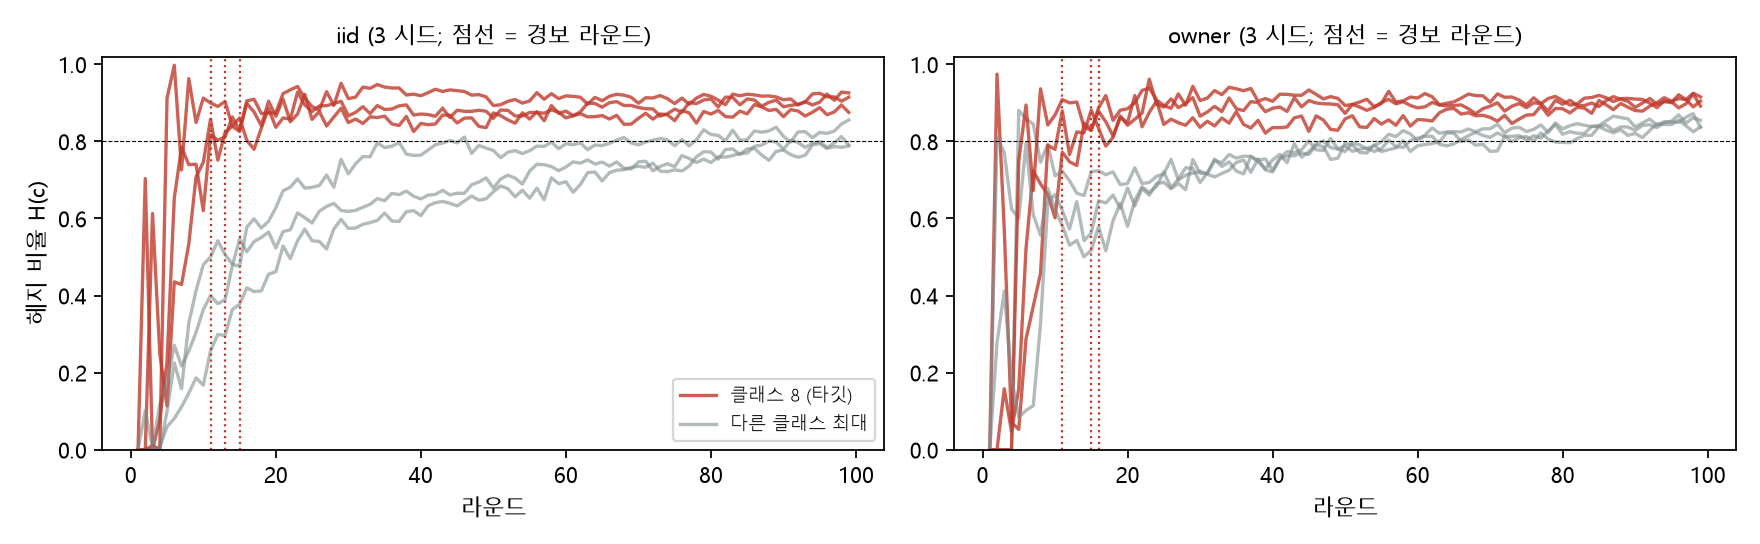
\includegraphics[width=\linewidth]{fig_H_curve.png}
\caption{라운드별 상쇄율. 클래스 8(빨강)은 10 라운드 안에 0.8을 넘고 끝까지 유지된다. 다른 클래스의 최대(회색)는 그 아래에 있다. 점선이 경보 라운드다.}
\label{fig:H}
\end{figure}

\begin{table}[t]\centering\small
\caption{기존 계열과 비교(R-009; 같은 6 궤적). ``잡힘'' = 숨기는 클라이언트를 1등으로 꼽은 시드 수. 소유자 $z$는 non-IID 조건.}
\label{tab:baselines}
\resizebox{\linewidth}{!}{%
\begin{tabular}{lccccc}\toprule
계열 (점수) & 잡힘 IID · non-IID & 소유자 $z$ & 심는 클라이언트 평균 순위/20 & 모델 생성 & 시점\\\midrule
갱신 크기: 노름 · Krum · 총노출 & 3/3 · 3/3 & 3.8 · 6.8 · 2.8 & 18.5 & 없음 & 학습 중\\
갱신 방향: 중앙값 코사인 · 반상관 · 누적 코사인 & 0/3 · 0/3 & 1.9 · 2.0 · 1.0 & 2.6--4.9 & 없음 & 학습 중\\
요청 심사, 절대 변화(20\% 빼기): 바뀐 답 · KL & 3/3 · 3/3 & 9.7 · 65.1 & 11--15 & 요청당 단계 수 & 요청 시\\
null-space 에너지 & 1/3 · 1/3 & $-9.9$ & 3--7 & 없음 & 요청 시\\
기능 효과: 타깃 몰림 · Fisher & 3/3 · 3/3 & $-1.8$ · 1.7 & 8--18 & 없음 & 요청 시\\
빼 보기, 상대 기준(flow $z$, 20\%) & 3/3 · 3/3 & 0.0 & 3.0--3.7 & 요청당 $K$개 & 요청 시\\
학습 중 부분합 감사(라운드 74) & 3/3 · 3/3 & 0.0 & 2.9--3.0 & 라운드당 $K$개 & 학습 중\\
참여 자연 실험(참여 회귀) & 3/3 · 3/3 & $-1.5$ & 15.0--15.2 & 없음 & 학습 중\\
\textbf{이 방법} & \textbf{3/3 · 3/3} & \textbf{제외 0/3} & \textbf{심는 넷 $=$ 올린 쪽 4/4} & \textbf{없음} & \textbf{13--14 라운드}\\
\bottomrule\end{tabular}}
\end{table}
\paragraph{기존 계열과 비교.} 표~\ref{tab:baselines}. 크기 기준은 소유자를 같이 잡고 심는 쪽을 가장 정상으로 본다. 방향 기준은 심는 쪽이 중심에 있어 못 본다. 숨기는 클라이언트만 잡는 것은 상대 기준 빼 보기, 기능 효과, 부분합 감사, 참여 회귀, 이 방법이고, 그중 심는 쪽까지 가리키고 모델 생성 없이 가장 이른 것은 이 방법이다.

\begin{table}[t]\centering\small
\caption{대응. 공격 성공률/정확도(\%), 요청자 = 숨기는 클라이언트.}
\label{tab:remedy}
\resizebox{\linewidth}{!}{%
\begin{tabular}{llll}\toprule
처방 & IID & non-IID & 출처\\\midrule
요청자만 빼고 처음부터 재학습(심는 쪽 남김) & 44.3$\pm$23.3 / 98.8 & 29.6$\pm$19.2 / 98.4 & $K=8$ 예비(R-001 설정)\\
증류 언러닝 & 18--25 / --- & --- & R-007\\
빼기 + 재억제 증류 & 5.6$\pm$2.2 / 96.0$\pm$0.4 (요청자 몫 0.09 되돌아옴) & --- & R-008\\
짝 몫 투영 제거(해독제) & 실패 & 실패 & R-011\\
\textbf{공모자 제외 재학습(처음부터)} & \textbf{0.5$\pm$0.1 / 99.0$\pm$0.0} & \textbf{0.6$\pm$0.2 / 98.9$\pm$0.0} & R-010\\
공모자 제외, 되돌아갈 라운드(13)에서 이어 학습 & 0.68 / 99.08 (노트북 1 시드) & \todo{R-014 예정} & R-014(예비)\\
공모자 제외, 경보 라운드(16)에서 바로 이어 학습 & 0.74 / 99.01 (노트북 1 시드) & \todo{R-014 예정} & R-014(예비)\\
\bottomrule\end{tabular}}
\end{table}
\paragraph{대응.} 표~\ref{tab:remedy}. 요청자를 완벽히 지우면 공격이 완성된다. 공모자를 빼야 성공률 0.5와 정확도 99가 같이 나온다. 되돌아가 이어 학습하는 것과 경보 즉시 빼는 것 모두 처음부터 재학습(노트북 기준 0.31)과 같은 수준이고 13--16 라운드를 아낀다.

\paragraph{문턱값 민감도.}\label{sec:sens} (R-013, 노트북 IID 1 시드, 저장된 영향으로 재판정.) 상쇄율 문턱 0.7/0.8/0.9 $\to$ 경보 13/16/65 라운드, 사람은 그대로. 내린 $z$ 문턱 5 $\to$ 22 라운드. 올린 $z$ 문턱 1.5 $\to$ 정상 한 명이 섞임(정밀도 0.8), 3 $\to$ 그대로. 연속 1 라운드 $\to$ 7 라운드에 정상을 가장 내린 사람으로 오판, 5 $\to$ 18 라운드. 최대 몫 1.0/0.6/0.5 $\to$ 학습 끝 오판 1/6 / 0/6 / 클래스 8 손상 1/6. 경보 시점은 문턱에 따라 움직이지만 누가 잡히는지는 연속 3 이상, 올린 $z$ 2 이상, 최대 몫 0.6--1에서 변하지 않는다.

\paragraph{비용.} 라운드당 9번 $\times$ 500장 순전파, 100 라운드 전체 1--2분(노트북 GPU). 요청 시점 심사(R-008)는 요청당 모델 280개, 빼 보기 546회. 대응은 87--93 라운드 학습 대 처음부터 100 라운드.

\section{한계}
\begin{itemize}
\item 공격 없는 궤적에서의 거짓 경보율을 아직 재지 않았다(R-015 예정). \S5의 두 번째 문단은 이 수치 없이는 주장이 아니다.
\item 이 방법은 상쇄가 공개 입력에 새는 공격만 본다. FUBA는 샌다. BadFU의 노트북 15 라운드 궤적에서는 새지 않았다(R-017, 경보 없음)---40 라운드 시드로 재확인하고, 새지 않으면 요청 시점 빼 보기로 보완한다.
\item 숨기는 클라이언트가 여럿인 경우, 다중 타깃, 집계 방어(Median·Multi-Krum·FLAME·FLDetector) 위의 궤적은 실측 전이다.
\item MNIST/LeNet이다. CIFAR-10/resnet18 궤적은 생성 중이다.
\end{itemize}

\section{결론}
삭제로 깨어나는 백도어는 같은 입력에 반대되는 학습 신호를 보내 평균에서 사라지게 한 것이다. 그 신호는 학습 중 각 클라이언트가 각 클래스를 얼마나 올리고 내렸는지에 남는다. 여럿이 올리고 한 명이 그만큼 내리는 클래스를 찾으면 타깃·숨기는 쪽·심는 쪽이 한 번에 나오고, 그들을 빼고 이어 학습하면 삭제는 이행되고 백도어는 사라진다.

\section*{부록. 결과 번호 $\leftrightarrow$ 표}
표 1 R-006 · 표 2 R-012, R-013 · 표 3 R-009 · 표 4 R-001($K=8$), R-007, R-008, R-010, R-011, R-014 · 민감도 R-013 · R-015(공격 없음), R-016(숨기는 쪽 2명), R-017(BadFU), R-018(CIFAR) 예정.
\end{document}
